%!TEX program = xelatex

% 纸张模式:护眼模式-geye 朦胧模式-hazy
% 纸张尺寸:pad kindle pc normal screen

\documentclass[cn, hazy, blue, normal, 14pt]{elegantnote}

\title{数字信号处理例题讲解}
\author{Xiaohei}
\version{1.0}
\date{\zhtoday}

\usepackage{tikz}
\usepackage{amssymb}
\usepackage{pgfplots}
\usepackage{bookmark}
\usepackage{multirow}
\usepackage{tabularx}
\usepackage[verbose]{xsim}

\tikzset{
    box/.style ={
        rectangle,              % 矩形节点
        rounded corners = 5pt,  % 圆角
        minimum width   = 50pt, % 最小宽度
        minimum height  = 20pt, % 最小高度
        inner sep = 5pt,        % 文字和边框的距离
        draw=blue               % 边框颜色
    }
}

\begin{document}

\maketitle

\setlength{\lineskip}{1.5em}
\setlength{\parskip}{0}


本文章为数字信号处理(电气)课程的部分例题讲解,由于部分答案为个人编撰,难免会出现部分错误,请保证使用GitHub仓库所发布的最新版本。如遇问题可在GitHub上发布Issue或直接联系我。


\section{离散时间信号与系统}


\begin{exercise}

一模拟信号$x_a(t)=\sin(240\pi t)+5\sin(360\pi t)$,采用300Hz的抽样频率进行采样。

\begin{quote}
\begin{itemize}
    \item[1)] 求信号的Nyquist抽样频率。
    \item[2)] 求信号的折叠频率。
    \item[3)] 求经过抽样后的序列$x(n)$。
    \item[4)] 若序列$x(n)$通过理想D/A进行转换,求转换后的信号$y_a(t)$。
\end{itemize}
\end{quote}

\end{exercise}

\begin{solution}[print=true]

1) 360Hz。Nyquist抽样频率为信号最高频率的2倍。

2) 150Hz。折叠频率为抽样频率的一半。

3) 采样后的序列$x(n)$为:

\begin{equation}
\notag
\begin{aligned}
    x(n)=x_a(nT_s)=x_a\left(\frac{n}{f_s}\right)&=\sin\left(240\pi\cdot\frac{n}{300}\right)+5\sin\left(360\pi\cdot\frac{n}{300}\right) \\
    &=\sin\left(0.8\pi n\right)+5\sin\left(1.2\pi n\right) \\
    &=\sin\left(0.8\pi n\right)-5\sin\left(2\pi n-1.2\pi n\right) \\
    &=-4\sin\left(0.8\pi n\right)
\end{aligned}
\end{equation}

4) 恢复后的信号$y_a(t)$为:

\begin{equation}
\notag
\begin{aligned}
    y_a(t)=x\left(\frac{t}{T_s}\right)=x(tf_s)&=-4\sin\left(0.8\pi \cdot 300 t\right) \\
    &=-4\sin\left(240\pi t\right)
\end{aligned}
\end{equation}

\end{solution}


\section{$z$变换与离散时间Fourier变换(DTFT)}

\begin{exercise}

已知离散LSI系统的差分方程

\begin{equation}
\notag
    y(n)-\frac{3}{4}y(n-1)+\frac{1}{8}y(n-2)=x(n)+\frac{1}{3}x(n-1)
\end{equation}

其中$x(n)$为输入,$y(n)$为输出。

\begin{quote}
\begin{itemize}
    \item[1)] 求系统函数,并指出零极点。
    \item[2)] 若该系统因果稳定,指出系统收敛域。
    \item[3)] 求该因果稳定系统的单位抽样响应。 
\end{itemize}
\end{quote}

\end{exercise}

\begin{solution}[print=true]
    
1) 对差分方程两边取$z$变换:

\begin{equation}
\notag
    Y(z)-\frac{3}{4}z^{-1}Y(z)+\frac{1}{8}z^{-2}Y(z)=X(z)+\frac{1}{3}z^{-1}X(z)
\end{equation}

则系统函数为:

\begin{equation}
\notag
    H(z)=\dfrac{Y(z)}{X(z)}=\dfrac{1+\dfrac{1}{3}z^{-1}}{1-\dfrac{3}{4}z^{-1}+\dfrac{1}{8}z^{-2}}=\dfrac{1+\dfrac{1}{3}z^{-1}}{\left(1-\dfrac{1}{2}z^{-1}\right)\left(1-\dfrac{1}{4}z^{-1}\right)}
\end{equation}

其零点为$z=-\dfrac{1}{3}, 0$,极点为$z=\dfrac{1}{2}, \dfrac{1}{4}$。(不要遗漏$z=0$的零点)

2) 由于系统为因果稳定系统,故其收敛域:

\begin{equation}
    \notag
    |z|>\frac{1}{2}
\end{equation}

3) 用部分分式法求$H(z)$的$z$变换:

\begin{equation}
    \notag
    H(z)=\dfrac{1+\dfrac{1}{3}z^{-1}}{\left(1-\dfrac{1}{2}z^{-1}\right)\left(1-\dfrac{1}{4}z^{-1}\right)}=\dfrac{\dfrac{10}{3}}{1-\dfrac{1}{2}z^{-1}}+\dfrac{-\dfrac{7}{3}}{1-\dfrac{1}{4}z^{-1}}
\end{equation}

根据$|z|>\dfrac{1}{2}$,通过查表法得:

\begin{equation}
    \notag
    h(n)=\left[\dfrac{10}{3}\left(\dfrac{1}{2}\right)^n-\dfrac{7}{3}\left(\dfrac{1}{4}\right)^n\right]u(n)
\end{equation}

\end{solution}


\section{离散Fourier变换(DFT)}

\begin{exercise}

设序列$x(n)$的傅氏变换为$X\left(\text{e}^{\text{j}\omega}\right)$,试求下列序列的傅立叶变换。

\begin{quote}
\begin{itemize}
    \item[1)] $x(2n)$。
    \item[2)] $x^*(n)$。
\end{itemize}
\end{quote}

\end{exercise}

\begin{solution}

1) 

\end{solution}

\begin{exercise}

对实信号进行谱分析,要求谱分辨率$F_0\leq 10\text{Hz}$,信号最高频率$f_h=2.5\text{kHz}$,试确定以下参量:

\begin{quote}
\begin{itemize}
    \item[1)] 最小记录长度$T_0$。
    \item[2)] 抽样点间的最大时间间隔$T$。
    \item[3)] 在一个记录中的最小抽样点数$N$。
\end{itemize}
\end{quote}

\end{exercise}

\begin{solution}[print=true]
    


\end{solution}

\begin{exercise}

若存在模拟信号

\begin{equation}
\notag
    x_a(t)=[\cos(160\pi t)+\cos(200\pi t)]\cos(1200\pi t)
\end{equation}

使用DFT做谱分析,要求能分辨该信号的所有频率分量,试求:

\begin{quote}
\begin{itemize}
    \item[1)] 最小采样频率$f_s$。
    \item[2)] 采样后的离散序列$x(n)$。
    \item[3)] 在一个记录中的最小抽样点数$N$。
    \item[4)] 使用1200Hz的采样频率对信号采样后通过理想D/A恢复的信号$x'_a(t)$。
\end{itemize}
\end{quote}

\end{exercise}

\begin{solution}[print=true]
    


\end{solution}


\section{快速Fourier变换(FFT)}




\section{数字滤波器的基本结构}

\begin{exercise}

已知系统由下面差分方程描述:

\begin{equation}
\notag
    y(n)=x(n)+\frac{1}{2}x(n-1)+\frac{5}{6}y(n-1)-\frac{1}{6}y(n-2)
\end{equation}

试画出系统的直接\uppercase\expandafter{\romannumeral1}型、直接\uppercase\expandafter{\romannumeral2}型、级联型和并联型结构。其中$x(n)$和$y(n)$分别表示系统的输入和输出信号。

\end{exercise}

\begin{solution}[print=true]

该IIR系统的系统函数为:

\begin{equation}
    H(z)=\dfrac{1+\dfrac{1}{2}z^{-1}}{1-\dfrac{5}{6}z^{-1}+\dfrac{1}{6}z^{-2}}=\dfrac{\sum\limits_{k=0}^{M}b_k z^{-k}}{1-\sum\limits_{k=1}^{N}a_k z^{-k}}
\end{equation}

可得$a_1=\dfrac{5}{6}$,$a_2=-\dfrac{1}{6}$,$b_0=1$,$b_1=\dfrac{1}{2}$。可画出直接\uppercase\expandafter{\romannumeral1}型和直接\uppercase\expandafter{\romannumeral2}型结构如图:

\begin{figure}[htbp]
\caption{直接\uppercase\expandafter{\romannumeral1}型}
\centering
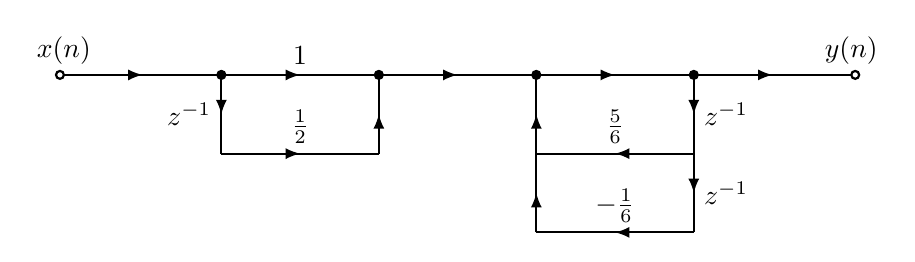
\begin{tikzpicture}[thick]
    \draw (1.95,3) circle [radius=0.05];
    \draw (12.05,3) circle [radius=0.05];
    \draw (2,3) -- (12,3);
    
    \filldraw (4,3) circle [radius=0.05];
    \filldraw (6,3) circle [radius=0.05];
    \filldraw (8,3) circle [radius=0.05];
    \filldraw (10,3) circle [radius=0.05];

    \draw[-latex] (2,3) -- (3,3);
    \draw[-latex] (4,3) -- (5,3);
    \draw[-latex] (6,3) -- (7,3);
    \draw[-latex] (8,3) -- (9,3);
    \draw[-latex] (10,3) -- (11,3);

    \draw (4,2) -- (6,2);
    \draw[-latex] (4,2) -- (5,2);
    \draw (10,1) -- (8,1);
    \draw[-latex] (10,1) -- (9,1);
    \draw (10,2) -- (8,2);
    \draw[-latex] (10,2) -- (9,2);

    \draw (4,3) -- (4,2);
    \draw (6,3) -- (6,2);
    \draw (8,3) -- (8,1);
    \draw (10,3) -- (10,1);

    \draw[-latex] (4,3) -- (4,2.5);
    \draw[-latex] (10,3) -- (10,2.5);
    \draw[-latex] (10,2) -- (10,1.5);

    \draw[-latex] (6,2) -- (6,2.5);
    \draw[-latex] (8,2) -- (8,2.5);
    \draw[-latex] (8,1) -- (8,1.5);
    
    \node[above] at (2,3) {$x(n)$};
    \node[above] at (12,3) {$y(n)$};

    \node[left] at (4,2.5) {$z^{-1}$};
    \node[right] at (10,1.5) {$z^{-1}$};
    \node[right] at (10,2.5) {$z^{-1}$};

    \node[above] at (5,3) {$1$};
    \node[above] at (5,2) {$\frac{1}{2}$};

    \node[above] at (9,2) {$\frac{5}{6}$};
    \node[above] at (9,1) {$-\frac{1}{6}$};

\end{tikzpicture}
\end{figure}

\begin{figure}[htbp]
\caption{直接\uppercase\expandafter{\romannumeral2}型}
\centering
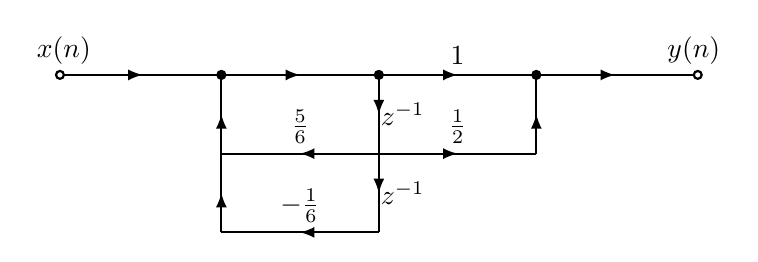
\begin{tikzpicture}[thick]
    \draw (1.95,3) circle [radius=0.05];
    \draw (10.05,3) circle [radius=0.05];
    \draw (2,3) -- (10,3);
    
    \filldraw (4,3) circle [radius=0.05];
    \filldraw (6,3) circle [radius=0.05];
    \filldraw (8,3) circle [radius=0.05];

    \draw[-latex] (2,3) -- (3,3);
    \draw[-latex] (4,3) -- (5,3);
    \draw[-latex] (6,3) -- (7,3);
    \draw[-latex] (8,3) -- (9,3);

    \foreach \i in {1,2}{
        \draw (6,\i) -- (4,\i);
        \draw[-latex] (6,\i) -- (5,\i);
    }

    \foreach \i in {2}{
        \draw (6,\i) -- (8,\i);
        \draw[-latex] (6,\i) -- (7,\i);
    }

    \foreach \i in {4,6}{
        \draw (\i,3) -- (\i,1);
    }

    \foreach \i in {8}{
        \draw (\i,3) -- (\i,2);
    }

    \foreach \i in {4}{
        \draw[-latex] (\i,2) -- (\i,2.5);
        \draw[-latex] (\i,1) -- (\i,1.5);
    }

    \foreach \i in {6}{
        \draw[-latex] (\i,3) -- (\i,2.5);
        \draw[-latex] (\i,2) -- (\i,1.5);
    }

    \foreach \i in {8}{
        \draw[-latex] (\i,2) -- (\i,2.5);
    }
    
    \node[above] at (2,3) {$x(n)$};
    \node[above] at (10,3) {$y(n)$};

    \foreach \i in {1.5,2.5}{
        \node[right=-3pt] at (6,\i) {$z^{-1}$};
    }

    \node[above] at (7,3) {$1$};
    \node[above] at (7,2) {$\frac{1}{2}$};

    \node[above] at (5,2) {$\frac{5}{6}$};
    \node[above] at (5,1) {$-\frac{1}{6}$};

\end{tikzpicture}
\end{figure}

级联和并联型的系统函数为:

\begin{equation}
\notag
    H(z)=\dfrac{1+\dfrac{1}{2}z^{-1}}{1-\dfrac{5}{6}z^{-1}+\dfrac{1}{6}z^{-2}}=\dfrac{1+\dfrac{1}{2}z^{-1}}{1-\dfrac{1}{2}z^{-1}}\cdot\dfrac{1}{1-\dfrac{1}{3}z^{-1}}=\dfrac{6}{1-\dfrac{1}{2}z^{-1}}-\dfrac{5}{1-\dfrac{1}{3}z^{-1}}
\end{equation}

结构流图即为分别实现子系统后级联或并联,形式不唯一,需要注意不要遗漏并联子系统的系数,图略。

\end{solution}


\section{IIR滤波器设计}

\begin{exercise}

用双线性变换法设计一个三阶数字Butterworth低通滤波器,采样频率$f_s=4\text{kHz}$,其3dB截止频率为$f_c=1\text{kHz}$,三阶模拟Butterworth低通滤波器为

\begin{equation}
\notag
    H_a(s)=\dfrac{1}{1+2\left(\dfrac{s}{\Omega_c}\right)+2\left(\dfrac{s}{\Omega_c}\right)^2+\left(\dfrac{s}{\Omega_c}\right)^3}
\end{equation}

\end{exercise}

\begin{solution}[print=true]

截止频率对应的数字频率$\omega_c$为

\begin{equation}
\notag
    \omega_c=2\pi  f_c T_s=2\pi f_c\dfrac{1}{f_s}=0.5\pi
\end{equation}

则$\Omega_c$为

\begin{equation}
\notag
    \Omega_c=c\tan\dfrac{\omega_c}{2}=c
\end{equation}

所以

\begin{equation}
\notag
    H_a(s)=\dfrac{1}{1+2\left(\dfrac{s}{c}\right)+2\left(\dfrac{s}{c}\right)^2+\left(\dfrac{s}{c}\right)^3}
\end{equation}

映射到$z$平面为

\begin{equation}
\notag
\begin{aligned}
    H(z)=\left.H_a(s)\right|_{s=c\frac{1-z^{-1}}{1+z^{-1}}}&=\dfrac{1}{1+2\left(\frac{1-z^{-1}}{1+z^{-1}}\right)+2\left(\frac{1-z^{-1}}{1+z^{-1}}\right)^2+\left(\frac{1-z^{-1}}{1+z^{-1}}\right)^3} \\
    &=\frac{1}{6}\cdot\frac{1+3z^{-1}+3z^{-2}+z^{-3}}{1+\frac{1}{3}z^{-2}}
\end{aligned}
\end{equation}

\end{solution}

\begin{exercise}

已知模拟滤波器的系统函数$H_a(s)=\dfrac{1}{2s^2+3s+1}$,用脉冲响应不变法和双线性变换法分别将其转化为数字滤波器,采样周期$T=2$秒。

\end{exercise}

\begin{solution}[print=true]
    


\end{solution}


\section{FIR滤波器设计}

\begin{exercise}

用矩形窗设计一个FIR线性相位低通数字滤波器。已知通带的截止频率$\omega_p=0.5\pi$,窗的长度$N=17$,求出$h(n)$的表达式即可。

\end{exercise}

\begin{solution}[print=true]



\end{solution}


\section{综合题}

\begin{exercise}

如图为一数字信号处理系统,其中A/D为模数转换器,$x(t)=\sin(200\pi t)+\sin(300\pi t)$为系统模拟输入信号,试解答如下问题:

\begin{center}
\begin{tikzpicture}
    \node[box] (1) at(2,0) {A/D};
    \node[box] (2) at(6.5,0) {数字信号处理器\textcircled{1}};
    \node[box] (3) at(11,0) {输出};
    \draw[->] (0, 0) -- (1);
    \draw[->] (1) -- (2);
    \draw[->] (2) -- (3);
    \node at(0.5,0.5) {$x(t)$};
    \node at(3.7,0.5) {$x(n)$};
\end{tikzpicture}
\end{center}

\begin{quote}
\begin{itemize}
    \item[1)] 若图中数字信号处理器\textcircled{1}是IIR数字滤波器并具有高通特性,试确定其截止频率和输出信号(忽略滤波器带来的影响)。
    \item[2)] 简要叙说IIR和FIR这两种滤波器的异同(至少涉及3个方面)。
    \item[3)] 设A/D采样率为512Hz,对序列$x(n)$进行256个点的FFT变换。求两谱线间的频率间隔。若对上述数据进行离散傅立叶反变换,则反变换后的抽样间隔是多少?整个256个点的时宽又为多少?
\end{itemize}
\end{quote}

\end{exercise}

\begin{solution}[print=true]



\end{solution}

\end{document}
